General process

- divide the dataset in train and test
Learning the parameters of a prediction function and testing it on the same data is a methodological mistake: a model that would just repeat the labels of the samples that it has just seen would have a perfect score but would fail to predict anything useful on yet-unseen data. This situation is called overfitting. To avoid it, it is common practice when performing a (supervised) machine learning experiment to hold out part of the available data as a test set.
- learn and evaluate
- feature description
- choose of the classifier

Feature description

presenting different channel representation
RGB, gray, HSV

Local binary pattern

Local binary pattern is a visual descriptor for texture composiiton of an image, first presented in .

Show an image and its LBP representation

% http://www.pyimagesearch.com/2015/12/07/local-binary-patterns-with-python-opencv/


Color histogram and moments :

mean and variance
Hu moment (+ raw and centralized and normalized moment and their property)
joint histogram

Cite + write formula

Bag-of-Words

Bag-of-Words, also called Bag of features, is a 
derived from text classification

cite who use it first?

overall process

Sift

Surf

Feature detection
- can use sift or surf
- dense grid (cite why it is better)

Descriptor

clustering
- k means

Classifier

k-nearest neighborhood

one of the simplest

Tree, random forest

Decision tree: can be used for classification or regression
It can be represented as a graph and a simple representation is given \ref{fig:decision_tree_simple_example}.

\begin{figure}[h]
    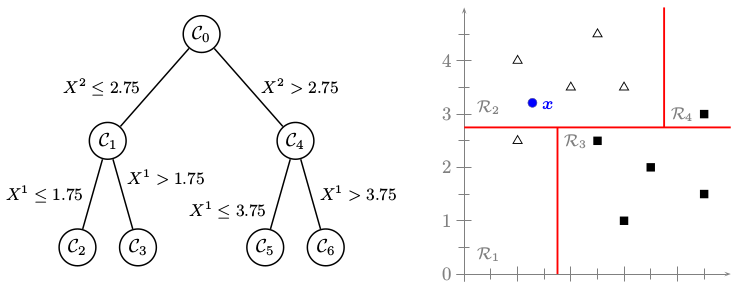
\includegraphics[scale=0.5]{img/decision_tree_simple_example}
    \caption{Decision tree of depth 2 for 10 elements belonging to 2 classes}
    \label{fig:decision_tree_simple_example}
\end{figure}


Naive bayesian

SVM (binary case) + kernel trick + multi-class (one-versus-one or one-versus-all)

Kernel trick:
to use the linear SVM for non-linear data: project the data in a new feature H space thanks to an application and then reserch for maximum margin hyperplan in H
to make sure that the new problem has a unique solution, 
must satisfy the Mercer's condition or simply it must be a positiv-definit matrix
give some "famous" kernel (chi2, rbf, polynomial)

cite the first to use kernel trick
cite why i use $\chi^2$

SGD classifier + loss function + regularization term% http://scikit-learn.org/stable/modules/sgd.html#mathematical-formulation

CNN

inspired by the neural system composed of different layers and communication shemes
recent years: use of the adjectiv "deep" to qualify NN: many layers

Different types of layers:
% http://cs231n.github.io/convolutional-networks/
% http://caffe.berkeleyvision.org/tutorial/layers.html
% Vision
- convolutional (give the name of the type of NN) : The Convolution layer convolves the input image with a set of learnable filters, each producing one feature map in the output image.
- max pooling
- normalization layer % http://stats.stackexchange.com/a/161200
% Loss layer
- sigmoid
% Activation / Neuron Layers
- ReLu